


\newpage
\section{diagram przypadkow uzycia}
\begin{figure}
\vspace{-2cm}
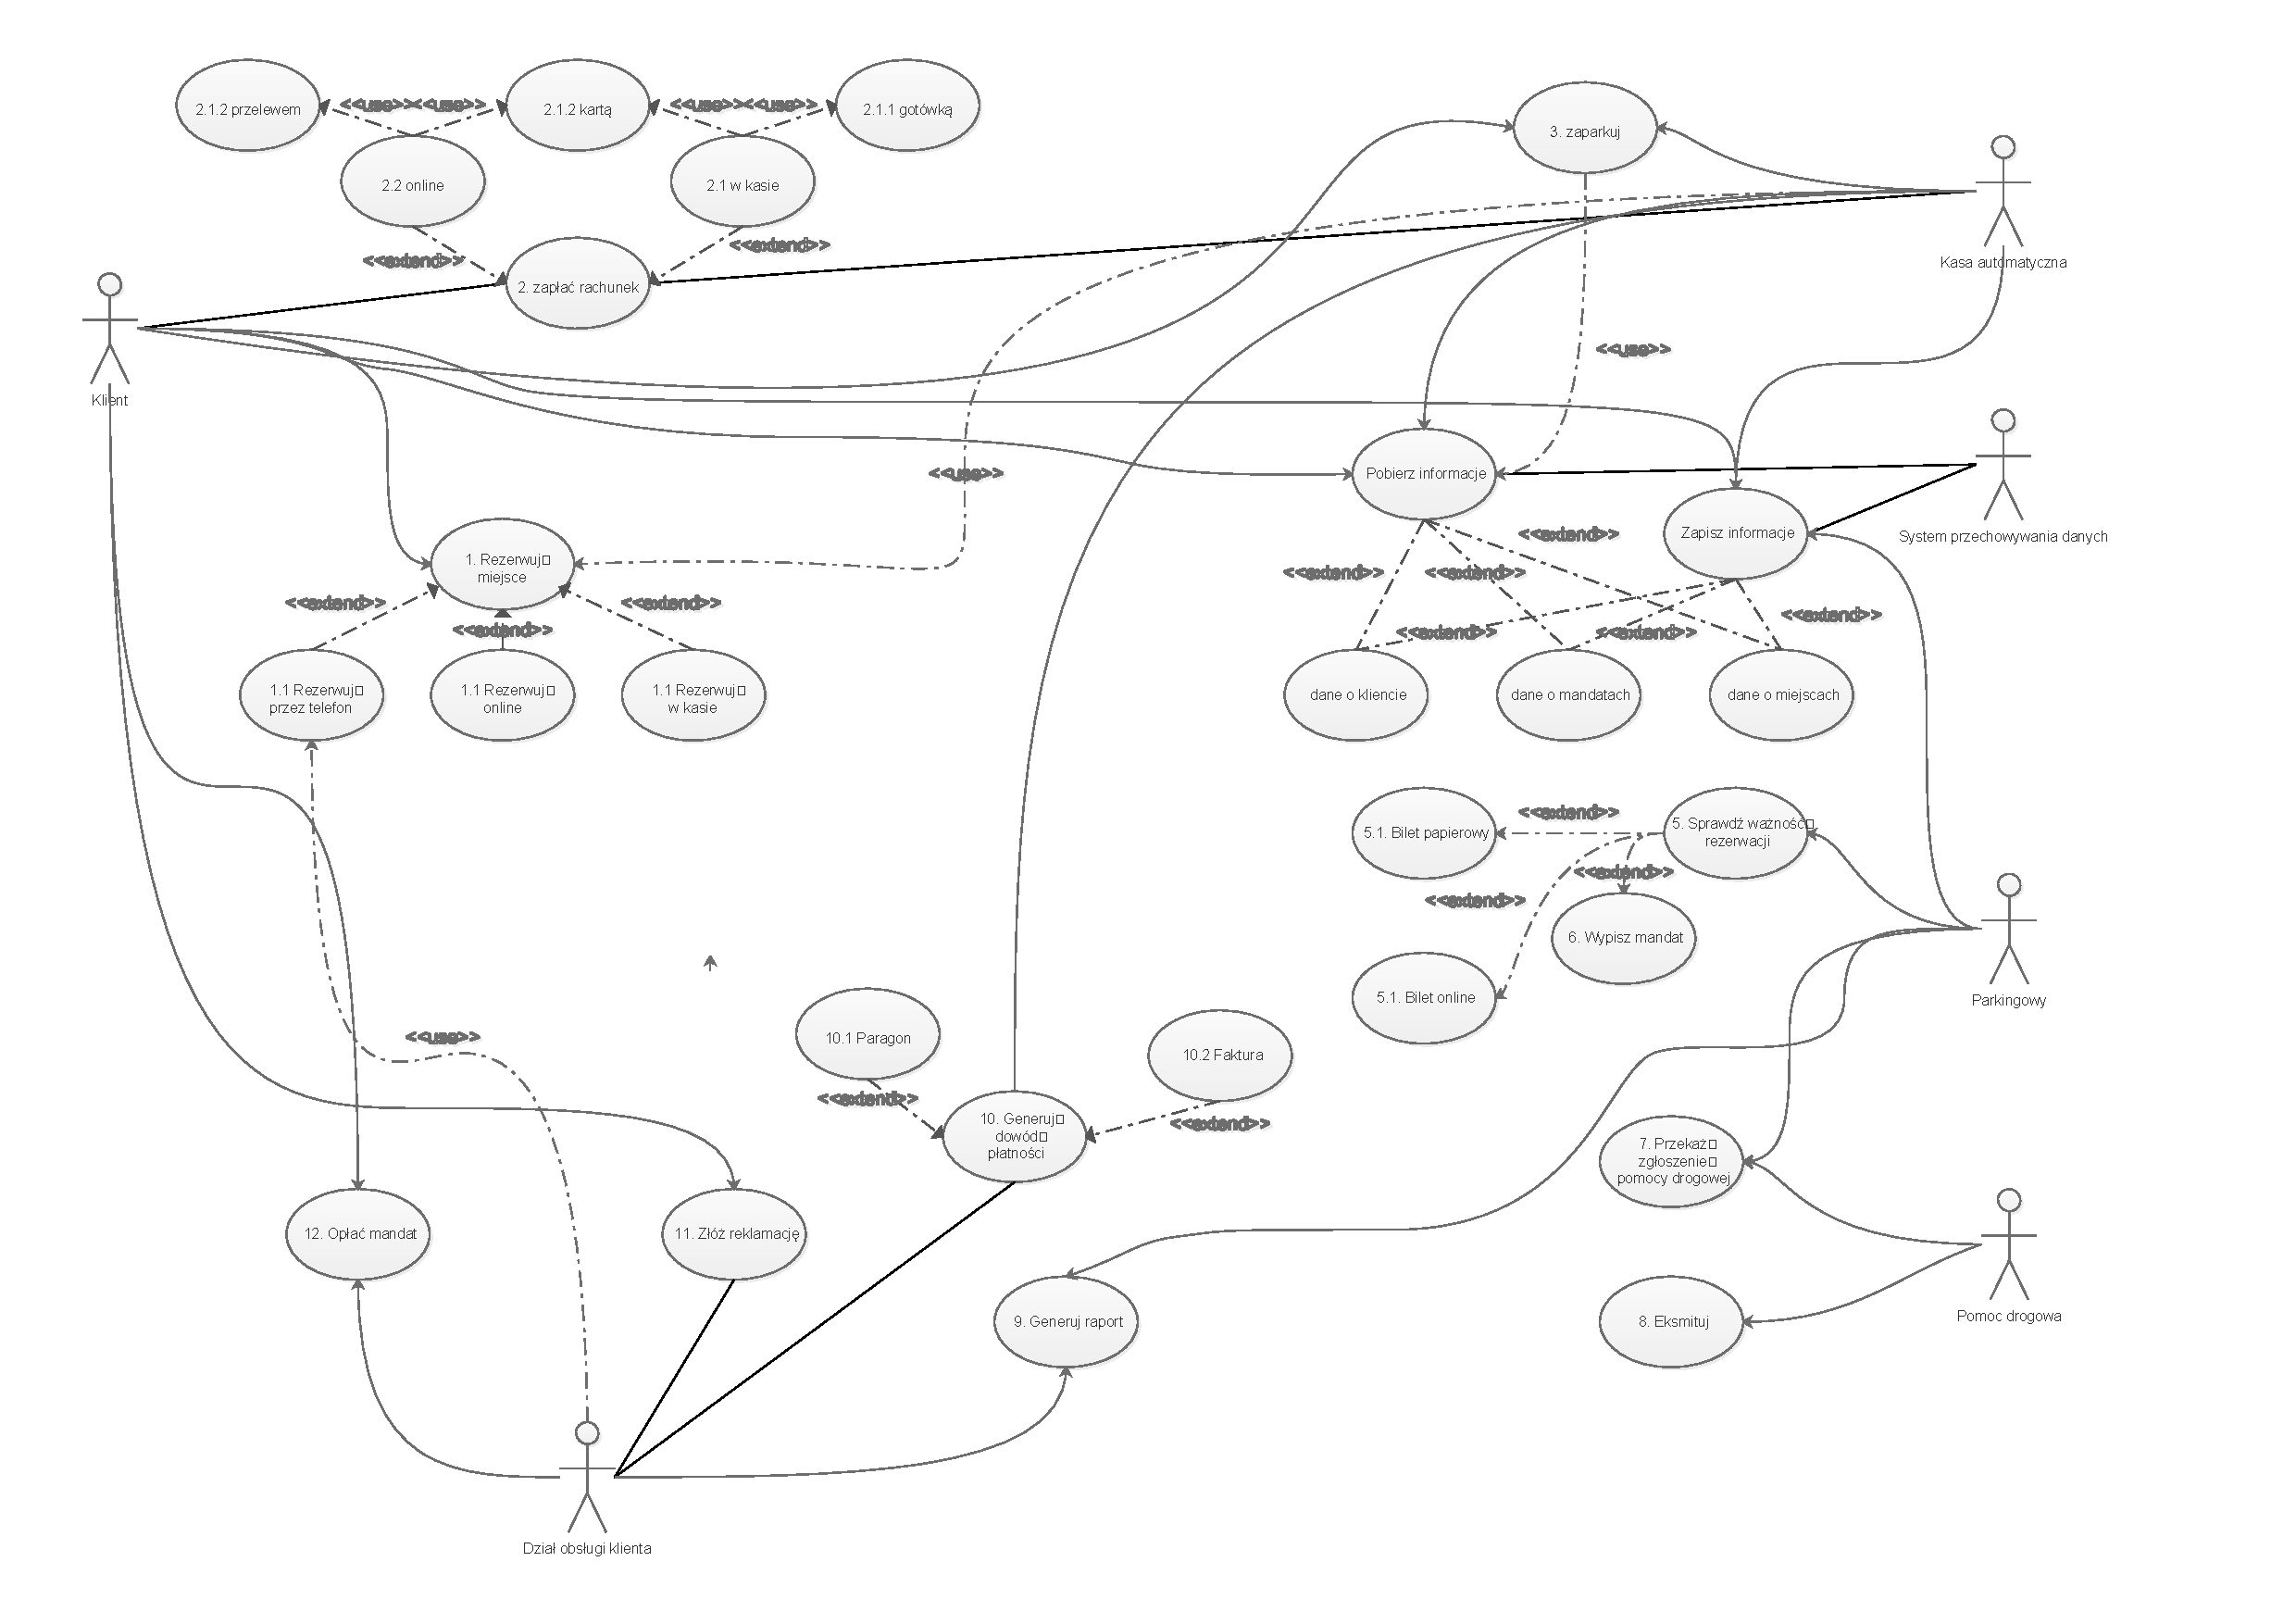
\includepdf[trim=0cm 0 0 -1cm]{uzycia/usecase}
\end{figure}
%\begin{landscape}
%\includegraphics[scale=0.65]{use-case}
%\end{landscape}

\newpage
\section{scenariusze przypadków użycia}
\begin{center}
\begin{tabular}{|L{3cm}  L{13cm}|}
\hline
Nazwa: & 1.1 Rezerwacja miejsca online - płatność kartą \\ \hline
Aktorzy: & Klient,  Automatyczna kasa \\ \hline
Podstawowy ciąg zdarzeń: & 1. Klient wchodzi na stronę www \\
 & 2. Klient wybiera datę i ilość godzin rezerwacji \\
 & 3. Klient zgłasza chęć zrobienia rezerwacji \\
 & 4. Automatyczna kasa rejestruje rezerwację \\
 & 5. Automatyczna kasa wysyła potwierdzenie zrobienia rezerwacji \\
 & 6. Klient dokonuje płatności kartą \\ \hline
Alternatywny ciąg zdarzeń:  & \# Klient rezygnuje z rezerwacji \\
 & \# Klient zmienia datę i ilość godzin w rezerwacji \\
 & \# Automatyczna kasa zwraca informację o braku miejsca w danym terminie\\ 
 \\ \hline
\end{tabular}

\vspace{1cm}

\begin{tabular}{|L{3cm}  L{13cm}|}
\hline
Nazwa: & 1.3 Rezerwacja miejsca online - płatność przelew \\ \hline
Aktorzy: & Klient,  Automatyczna kasa \\ \hline
Podstawowy ciąg zdarzeń: & 1. Klient wchodzi na stronę www \\
 & 2. Klient wybiera datę i ilość godzin rezerwacji \\
 & 3. Klient zgłasza chęć zrobienia rezerwacji \\
 & 4. Automatyczna kasa rejestruje rezerwację \\
 & 5. Automatyczna kasa wysyła potwierdzenie zrobienia rezerwacji \\
 & 6. Klient dokonuje płatności przelewem \\ \hline
Alternatywny ciąg zdarzeń:  & \# klient rezygnuje z rezerwacji \\
 & \# klient zmienia datę i ilość godzin w rezerwacji \\ 
 & \# Automatyczna kasa zwraca informację o braku miejsca w danym terminie\\ \hline
\end{tabular}

\vspace{1cm}

\begin{tabular}{|L{3cm}  L{13cm}|}
\hline
Nazwa: & 1.4 Rezerwacja na miejscu - płatność kartą \\ \hline
Aktorzy: & Klient,  Automatyczna kasa \\ \hline
Podstawowy ciąg zdarzeń: & 1. Klient przyjeżdza na parking \\
 & 2. Klient wybiera długość postoju \\
 & 4. Automatyczna kasa rejestruje rezerwację \\
 & 5. Automatyczna kasa pokazuje informację o dostępności miejsc \\
 & 6. Klient dokonuje płatności kartą \\
 & 7. Automatyczna kasa generuje potwierdzenie zapłaty - paragon \\ \hline
Alternatywny ciąg zdarzeń:  & \# klient rezygnuje z rezerwacji \\
 & \# klient zmienia ilość godzin w rezerwacji \\ 
 & \# Automatyczna kasa zwraca informację o aktualnym braku miejsca\\ 
 & \# Automatyczna kasa zwraca informację o braku środków na koncie \\ \hline
\end{tabular}

\vspace{1cm}

\begin{tabular}{|L{3cm}  L{13cm}|}
\hline
Nazwa: & 1.5 Rezerwacja na miejscu - płatność gotówką \\ \hline
Aktorzy: & Klient,  Automatyczna kasa \\ \hline
Podstawowy ciąg zdarzeń: & 1. Klient przyjeżdza na parking \\
 & 2. Klient wybiera długość postoju \\
 & 4. Automatyczna kasa rejestruje rezerwację \\
 & 5. Automatyczna kasa pokazuje informację o dostępności miejsc \\
 & 6. Klient dokonuje płatności gotówką \\
 & 7. Automatyczna kasa generuje potwierdzenie zapłaty - paragon \\ \hline
Alternatywny ciąg zdarzeń:  & \# klient rezygnuje z rezerwacji \\
 & \# klient zmienia ilość godzin w rezerwacji \\ 
 & \# Automatyczna kasa zwraca informację o aktualnym braku miejsca\\ \hline
\end{tabular}

\vspace{1cm}

\begin{tabular}{|L{3cm}  L{13cm}|}
\hline
Nazwa: & 3 Zaparkowanie pojazdu \\ \hline
Aktorzy: & Klient,  Automatyczna kasa \\ \hline
Podstawowy ciąg zdarzeń: & 1. Klient zgłasza chęć odebrania rezerwacji miejsca w kasie automatycznej\\
 & 2. Kasa automatyczna przydziela klientowi wolne miejsce\\
 & 3. Klient parkuje pojazd w określonym miejscu\\ \hline
Alternatywny ciąg zdarzeń:  & \# klient rezygnuje z rezerwacji \\
 & \# Automatyczna kasa zwraca informację o braku miejsca\\ \hline
\end{tabular}

\vspace{1cm}

\begin{tabular}{|L{3cm}  L{13cm}|}
\hline
Nazwa: & 4. Sprawdzenie dostępności miejsca przez WWW \\ \hline
Aktorzy: & Klient,  Automatyczna kasa \\ \hline
Podstawowy ciąg zdarzeń: & 1. Klient wchodzi na stronę WWW \\
 & 2. Klient wybiera opcję sprawdzenia miejsca \\
 & 3. Automatyczna kasa sprawdza dostępne miejsca \\
 & 4. Automatyczna kasa zwraca informację do WWW \\ \hline
\end{tabular}

\vspace{1cm}

\begin{tabular}{|L{3cm}  L{13cm}|}
\hline
Nazwa: & 5.1 Sprawdzenie ważności biletu - bilet papierowy - bilet nie ważny krótką chwilę\\ \hline
Aktorzy: & Parkingowy, Klient \\ \hline
Podstawowy ciąg zdarzeń: & 1. Parkingowy sprawdza stan biletu papierowego w samochodzie klienta \\
 & 2  Parkingowy dzwoni do klienta aby uzyskać od niego informacje\\
 & 3.1 Parkingowy czeka na klienta \\
 & 3.2 Parkingowy wystawia mandat \\
 & 3.2. Parkingowy zapisuje mandat w systemie \\
 \hline
\end{tabular}

\vspace{1cm}

\begin{tabular}{|L{3cm}  L{13cm}|}
\hline
Nazwa: & 5.2 Sprawdzenie ważności biletu - bilet online - bilet nie ważny krótką chwilę\\ \hline
Aktorzy: & Parkingowy, Klient \\ \hline
Podstawowy ciąg zdarzeń: & 1. Parkingowy sprawdza stan biletu online w systemie poprzez wpisanie numeru rejestracyjnego klienta \\
 & 2  Parkingowy dzwoni do klienta aby uzyskać od niego informacje\\
 & 3.1 Parkingowy czeka na klienta \\
 & 3.2 Parkingowy wystawia mandat \\
 & 3.2 Parkingowy zapisuje mandat w systemie \\
 \hline
\end{tabular}

\vspace{1cm}

\begin{tabular}{|L{3cm}  L{13cm}|}
\hline
Nazwa: & 7 Eksmisja pojazdu\\ \hline
Aktorzy: & Parkingowy, Pomoc drogowa \\ \hline
Podstawowy ciąg zdarzeń: & 1. Parkingowy stwiedza nie opłaconą rezerwację oraz brak kontaktu z klientem\\
 & 2 Parkingowy dzwoni po pomoc drogową\\
 & 3 Pomoc drogowa odholowuje pojazd klienta \\
 \hline
\end{tabular}

\vspace{1cm}

\begin{tabular}{|L{3cm}  L{13cm}|}
\hline
Nazwa: & 9.1 Generowanie raportu miesięcznego przychodów\\ \hline
Aktorzy: & Dział obsługi klienta \\ \hline
Podstawowy ciąg zdarzeń: & 1.  Dział obsługi klienta zostaje powiadomiony o konieczności wygenerowania raportu za dany miesiąc\\
 & 2. Dział obsługi klienta generuje raport z systemu\\
 & 3. Dział obsługi klienta analizuje raport i dopisuje komentarz \\
 \hline
\end{tabular}

\vspace{1cm}

\begin{tabular}{|L{3cm}  L{13cm}|}
\hline
Nazwa: & 9.2 Generowanie raportu miesięcznych wystawionych mandatów\\ \hline
Aktorzy: & Parkingowy \\ \hline
Podstawowy ciąg zdarzeń: & 1. Parkingowy zleca wygenerowanie raportu wystawionych mandatów do systemu\\
 & 2. Parkingowy sprawdza poprawność ze stanem faktycznym za dany miesiąc\\
 & 3. Parkingowy dodaje komentarz, podpisuje dokument\\
 \hline
\end{tabular}


\vspace{1cm}

\begin{tabular}{|L{3cm}  L{13cm}|}
\hline
Nazwa: & 10. Wystawianie faktur za dany okres klientom biznesowym \\ \hline
Aktorzy: & Klient,  Dział obsługi klienta \\ \hline
Podstawowy ciąg zdarzeń: & 1. Klient żąda wydania faktury za dany okres \\
 & 2. Dział obsługi klienta generuje fakturę \\
 & 4. Dział obsługi klienta wysyła fakturę do klienta online \\ \hline
Alternatywny ciąg zdarzeń:  & \# klient rezygnuje z rezerwacji \\
 & \# akcja zapoczątkowana zdarzeniem z timera (generowanie faktury raz w miesiącu) \\ \hline
\end{tabular}

\vspace{1cm}

\begin{tabular}{|L{3cm}  L{13cm}|}
\hline
Nazwa: & 11.1 Klient składa reklamację online\\ \hline
Aktorzy: & Klient, Dział obsługi klienta \\ \hline
Podstawowy ciąg zdarzeń: & 1. Klient wchodzi na stronę WWW \\
 & 2. Klient wypełnia i wysyła formularz reklamacyjny \\
 & 3. Dział obsługi klienta rozpatruje reklamację w ciągu 30 dni robocznych\\
 & 4. Dział obsługi klienta wysyła zawiadomienie o rozpatrzeniu reklamacji \\
 \hline
Alternatywny ciąg zdarzeń:  & \# klient rezygnuje ze składania reklamacji \\
 & \# Dział obsługi klienta powiadamia klienta o zwiększeniu czasu rozpatrywania reklamacji \\ 
 \hline
\end{tabular}

\vspace{1cm}

\begin{tabular}{|L{3cm}  L{13cm}|}
\hline
Nazwa: & 11.2 Klient składa reklamację na miejscu\\ \hline
Aktorzy: & Klient, Dział obsługi klienta \\ \hline
Podstawowy ciąg zdarzeń: & 1. Klient przychodzi do działu obsługi klienta \\
 & 2. Klient wypełnia formularz reklamacyjny \\
 & 3. Pracownik działu obsługi klienta rozpatruje reklamację na miejscu \\
 & 4. Pracownik działu obsługi klienta informuje klienta o rozpatrzeniu reklamacji \\
 \hline
Alternatywny ciąg zdarzeń:  & \# Dział obsługi klienta powiadamia klienta o zwiększeniu czasu rozpatrywania reklamacji \\ 
 \hline
\end{tabular}

\vspace{1cm}

\begin{tabular}{|L{3cm}  L{13cm}|}
\hline
Nazwa: & 12.1 Opłacenie mandatu - paragon\\ \hline
Aktorzy: & Klient,  Dział obsługi klienta \\ \hline
Podstawowy ciąg zdarzeń: & 1. Klient przychodzi do działu obsługi klienta \\
 & 2. Klient przekazuje mandat pracownikowi działu obsługi klienta \\
 & 3. Pracownik działu obsługi klienta przyjmuje płatność od klienta \\
 & 4. Pracownik działu obsługi klienta wystawia paragon opłacenia mandatu \\
 & 5. Pracownik działu obsługi klienta wydaje kartę wyjazdową klientowi \\
 \hline
Alternatywny ciąg zdarzeń:  & \# Klient odmawia przyjęcia mandatu, składa reklamację \\ 
 \hline
\end{tabular}

\vspace{1cm}

\begin{tabular}{|L{3cm}  L{13cm}|}
\hline
Nazwa: & 12.2 Opłacenie mandatu - faktura\\ \hline
Aktorzy: & Klient,  Dział obsługi klienta \\ \hline
Podstawowy ciąg zdarzeń: & 1. Klient przychodzi do działu obsługi klienta \\
 & 2. Klient przekazuje mandat pracownikowi działu obsługi klienta \\
 & 3. Pracownik działu obsługi klienta przyjmuje płatność od klienta \\
 & 4. Pracownik działu obsługi klienta wystawia fakturę opłacenia mandatu \\
 & 5. Pracownik działu obsługi klienta wydaje kartę wyjazdową klientowi \\
 \hline
Alternatywny ciąg zdarzeń:  & \# Klient odmawia przyjęcia mandatu, składa reklamację \\ 
 \hline
\end{tabular}
\end{center}